%!TEX root = head-full.tex

\section{Partition Function Estimation} \label{sec:rbm}


\subsection{Restricted Bolztmann Machine}
Co-invented and enhanced largely\cite{hinton2006reducing} by Geoff Hinton, a Restricted Bolzmann Machine(RBM)\cite{mcclelland1987parallel} is a model which brings the idea of a physics concept to the field of computer science.

\begin{figure*}[tb]
% \vspace{-0.5in}
  	\centering
  	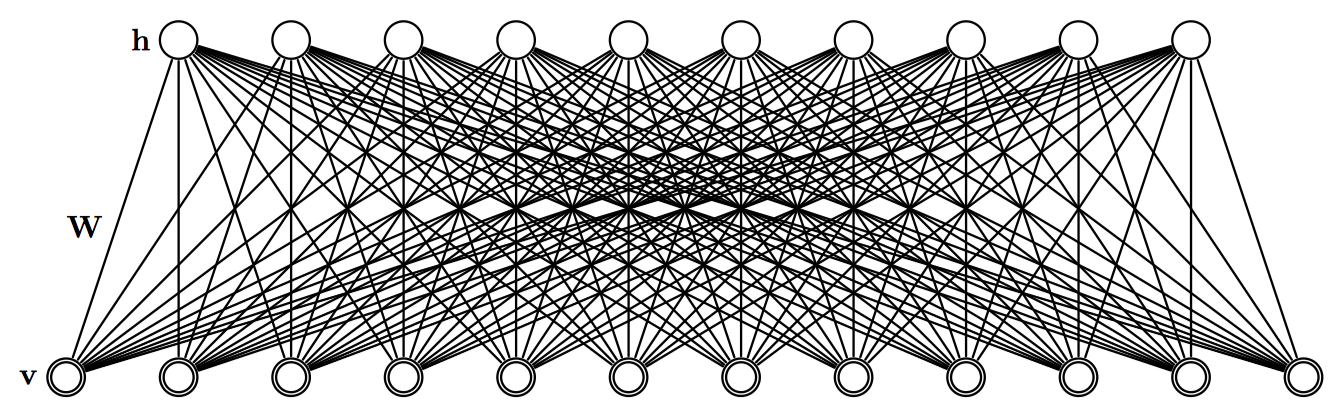
\includegraphics[width=1\textwidth]{figure/rbm.png}
% \vspace{-0.2in}
	\caption{A Restricted Boltzmann Machine}
	\label{fig:rbm}
\end{figure*}

\subsubsection{Introduction}
An RBM is a two-layer undirected model(Figure~\ref{fig:rbm}). The first layer of the RBM is called visible layer, and the second is called the hidden layer. In the model, every visible units are connected to all hidden units and vice versa. For every given value of visible layer $\mathbf v$ \& hidden layer $\mathbf h$, we can define an energy of this state.
\begin{equation}
E(\mathbf v,\mathbf h;\theta)=-\mathbf v^T\mathbf W\mathbf h-\mathbf b^T\mathbf v-\mathbf a^T\mathbf h
\end{equation}
where $\theta =\{W,\mathbf b,\mathbf a\}$ are the model configurations. $W_{ij}$ represents the weight between visible unit $v_{i}$ and hidden unit $h_{j}$. $\mathbf b$ \& $\mathbf a$ are biases for visible and hidden layer, respectively.

\subsubsection{Training an RBM}
On training an RBM, we want our RBM model to have a lowest scale of energy. By doing so, we have to calculate the joint distribution over the visible and hidden units, which is defined by:
\begin{equation}
	p(\mathbf v,\mathbf h;\theta)=\frac{e^{-E(\mathbf v,\mathbf h;\theta)}}{Z(\theta)}
\end{equation}
where
\begin{equation}
	Z(\theta)=\sum_{\mathbf v} \sum_{\mathbf h} e^{-E(\mathbf v,\mathbf h;\theta)}
\end{equation}
is the partition function.

However, calculating partition functions has always been an intractable work since we have to traverse all the possible state of $\mathbf v$ \& $\mathbf h$.
When the model grows large, this process will be very time \& rescouces consuming and thus become unrealistic for the real practice.

So, we have to introduce methods to estimate the partition functions instead of just calculating it in brute force. Although some deviation may include in the estimation, but the efficiency along with them make them preferable. In fact, studies have shown that only few deviation is included that we could just ignore it since it does petty influence on our training.

In the next subsection, we will discuss about three methods available, which each have their pros and cons in doing this complex estimation.



\subsection{Algorithms}

%!TEX root = RBM.tex

\subsubsection{Thouless-Anderson-Palmer Sampling\protect\footnote{Available at \protect\url{https://github.com/lzhbrian/MCMC/blob/master/rbm/TAP.m} in Matlab}}
Thouless-Anderson-Palmer Sampling(TAP)\cite{gabrie2015training} is a very efficient and easy-to-practice iterative procedure based on an improved mean field method from statistical physics called Thouless-Anderson-Palmer approach.

The main idea of this method is to iteratively compute the magnetization vector $m^{v}$,$m^{h}$, and then input the values into the Legendre transform of the free energy $F=log(Z(\theta))$ to compute it.

The Legendre transform of $F$ to the second order is:
\begin{equation}
\begin{split}
\Gamma(\mathbf m^{v},\mathbf m^{h}) &\approx - S(\mathbf m^{v},\mathbf m^{h}) - \sum_{i} a_{i}m^{v}_{i} - \sum_{j} b_{j}m^{h}_{j} \\
& - \sum_{i,j} \Bigg( W_{i,j}m^{v}_{i}m^{h}_{j} \\
& - 0.5W_{ij}\Big(m^{v}_{i}-(m^{v}_{i})^2\Big)\Big(m^{h}_{j}-(m^{h}_{j})^2\Big) \Bigg)
\end{split}
\end{equation}
where $S(\mathbf m^{v},\mathbf m^{h})$ indicates the entropy:
\begin{equation}
\begin{split}
S(\mathbf m^{v},\mathbf m^{h}) &= - \sum_{i} \Bigg(m^{v}_{i}logm^{v}_{i} + (1-m^{v}_{i})log(1-m^{v}_{i}) \Bigg) \\
&- \sum_{j} \Bigg(m^{h}_{j}logm^{h}_{j} + (1-m^{h}_{j})log(1-m^{h}_{j}) \Bigg)
\end{split}
\end{equation}

The pseudo code of this algorithm is shown below:


%!TEX root = RBM.tex

\subsubsection{Annealed Importance Sampling\protect\footnote{Available at \protect\url{https://github.com/lzhbrian/MCMC/blob/master/rbm/AIS.m} in Matlab}}
Annealed Importance Sampling(AIS)\cite{neal2001annealed,salakhutdinov2009learning} is probably one of the most preferable estimating methods avaible.

Previous work \cite{mackay2003information} have shown that if $P_{A}$ and $P_{B}$ in the SIS method is not close enough, the estimator would be very poor.

Based on SIS, the main idea of this algorithm is to gradually alter the value from an known $Z_{A}$ to our required $Z_{B}$ (or $Z_{K}$), by the following identity:
\begin{equation}
\frac{Z_{K}}{Z_{0}} = \frac{Z_{1}}{Z_{0}} \frac{Z_{2}}{Z_{1}} ... \frac{Z_{K}}{Z_{K-1}}
\end{equation}
where 
\begin{equation}
\frac{Z_{K}}{Z_{k+1}} = \frac{1}{M} \sum_{i=1}^{M} \frac{P_{k+1}^{*}(\mathbf x^{(i)})}{P_{k}^{*}(\mathbf x^{(i)})}
~~where~ x^{(i)} \sim P_{k}
\end{equation}
in which we can get $x_{k+1}$ from:
\begin{equation}
\begin{aligned}
p(h^{A}_{j}=1|\mathbf v) &= sigmoid\Bigg( (1-\beta_{k})\Bigg(\sum_{i}W^{A}_{ij}v_{i}+a^{A}_{j}\Bigg) \Bigg) \\
p(h^{B}_{j}=1|\mathbf v) &= sigmoid\Bigg( \beta_{k}\Bigg(\sum_{i}W^{B}_{ij}v_{i}+a^{B}_{j}\Bigg) \Bigg) \\ 
p(v'_{i}=1|\mathbf h) &= sigmoid\Bigg( (1-\beta_{k})\Bigg(\sum_{j}W^{A}_{ij}h_{i}^{A}+b^{A}_{i}\Bigg) \\
& + \beta_{k}\Bigg(\sum_{j}W^{B}_{ij}h_{j}^{B}+b^{B}_{i}\Bigg) \Bigg) 
\end{aligned}
\end{equation}
this procedure is shown in Figure~\ref{fig:xkxk1}.

\begin{figure}[tb]
% \vspace{-0.5in}
  	\centering
  	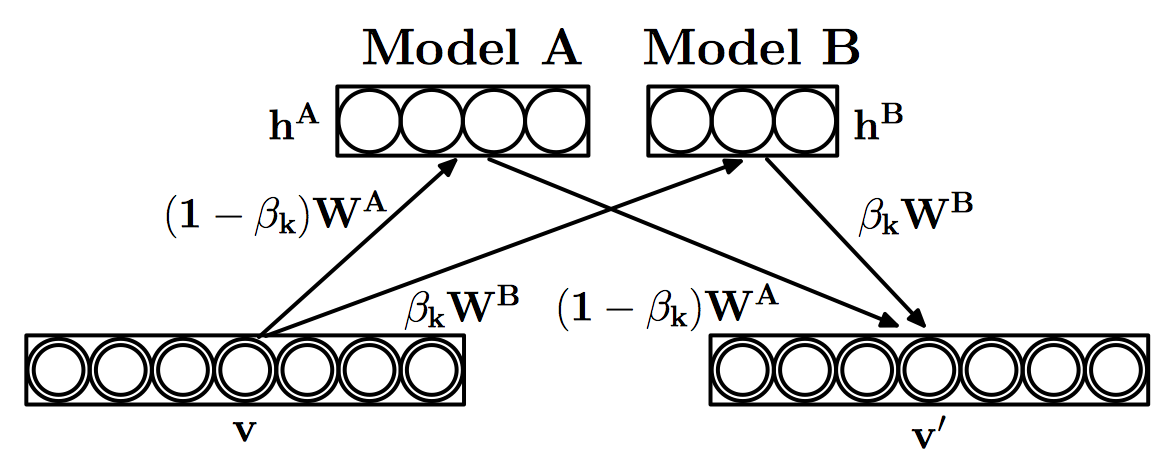
\includegraphics[width=0.4\textwidth]{figure/xkxk1.png}
% \vspace{-0.2in}
	\caption{The transition process from $x_{k}$ to $x_{k+1}$ which leaves $P_{k}(\mathbf v)$ invariant.}
	\label{fig:xkxk1}
\end{figure}

Note that model A indicates an initial model which we can easily compute all its configurations.

$\mathbf \beta$ in the above equations is defined by users as a set of inverse temperatures $\{0= \beta_{1} < \beta_{2} < ... < \beta_{K} =1\}$, which can define a sequence of
\begin{equation}
P_{k}(\mathbf x) \propto P_{A}^{*}(\mathbf x)^{1-\beta_{k}} P_{B}^{*}(\mathbf x)^{\beta_{k}}
\end{equation}
where 
\begin{equation}
P^{*}_{k}(\mathbf v)=\sum_{h^{A}h^{B}}e^{(1-\beta_{k})E(\mathbf v, \mathbf h^{A};\theta_{A})+\beta_{k}E(\mathbf v,\mathbf h^{B};\theta_{B})}
\end{equation}


The pseudo code of this algorithm is shown below:


%!TEX root = RBM.tex

\subsubsection{Rao-Blackwellized Tempered Sampling\protect\footnote{Available at \protect\url{https://github.com/lzhbrian/MCMC/blob/master/src/partition/RTS.m} in Matlab}}

\para{Algorithm}
Similar to AIS, Rao-Blackwellized Tempered (RTS)\cite{carlson2016partition} Sampling also has a set of inverse temperatures $\{0= \beta_{1} < \beta_{2} < ... < \beta_{K} =1\}$, which can define a sequence of
\begin{equation}
f_{k}(\mathbf x) \propto f(\mathbf x)^{\beta_{k}} p_{1}(\mathbf x)^{1-\beta_{k}}
\end{equation}

Different from AIS, we do not traverse $\mathbf \beta$. Instead we sample a $\beta^{*}$ every loop, from the $\mathbf \beta$ set with the distribution $(\beta|x)$.

Subsequently, we sample from $x_{k}$ to $x_{k+1}$ by the probability of $q(x|\beta^{*})$ just like what we did in AIS, shown in Figure~\ref{fig:xkxk1}. However, what also different from AIS is that, we have to iterate from $x_{k}$ to $x_{k+1}$ many times(i.e. 50 times in\cite{carlson2016partition} ) for the sake of getting a better $x_{k+1}$.

At the last of every loop, we update the lower variance estimator $\hat{\mathbf c}$ by
\begin{equation}
\hat{c}_{k} = \hat{c}_{k} + \frac{1}{N}q(\beta_{k}|x)
\end{equation}

Finally, we get $Z_{k}$ by
\begin{equation}
\hat{Z}_{k}^{RTS} = \hat{Z}_{k}\frac{r_{1}\hat{c}_{k}}{r_{k}\hat{c}_{1}},~~k=2,...,K
\end{equation}
in which what we do care is $Z_{B} \approx \hat{Z}_{K}^{RTS}$.

The posterier distribution $q(\beta_{k}|x)$ in the above equations is defined by:
\begin{equation}
q(\beta_{k}|x) = \frac{f_{k}(x)r_{k}/\hat{Z}_{k}}{\sum_{k'=1}^{K} f_{k'}(x)r_{k'}/\hat{Z}_{k'}}
\end{equation}

\para{Practice}
In the paper\cite{carlson2016partition}, Carlson et al. note an initializing method to initialize $Z_{k}$, whose procedure is just like the above process. The only difference is that they sampled $\beta_{k}$ by uniform distribution in every loop, not by the distribution $(\beta|x)$. They claim that after doing such initializing work, then we conduct the algorithms above would acquire a better result.

In our real practice, we directly use the initializing method mentioned above by selecting $\beta_{k}$ with a uniform distribution in every loop. We also initialize the value of $Z_{A}$ by the method we have mentioned in the AIS section using the dataset. And we have found that the result is already satisfying, there is no need to conduct more loops with $\beta_{k}$ sampled by $(\beta|x)$.

Also, we found that we have to conduct the procedure above for several times s.t. we can acquire our desired partition function value.(i.e. We did it for 100 times, that is to say we update $\mathbf Z$ for 100 times).

	\begin{algorithm}
        \caption{Rao-Blackwellized Tempered Sampling}
        \begin{algorithmic}
        	\Require $\{\beta_{k},r_{k}\}_{k=1,...,K}$
            \State Initialize $b_{A}$ by dataset
        	\State Initialize $log \hat{Z}_{k}, k=2,...,K$ 
            \For{$n = 1 \to Runtime$}
            	\State Initialize $\beta \in \{\beta_{1}...\beta_{K}\}$
            	\State Initialize $\hat{c}_{k}=0, k=1,...,K$
                \For{$t = 1 \to N$}
                    \For{$t = 1 \to Transition time$}
                        \State Sample $\mathbf x_{k+1}$ given $\mathbf x_{k}$ using $q(x|\beta^{*})$
                    \EndFor
                    \State $\mathbf x^{*} \gets \mathbf x_{k+1}$
    	            \State Sample $\beta^{*} \sim (\beta|\mathbf x^{*})$ or $\beta^{*} \in \{\beta_{1}...\beta_{K}\}$
    	            \State Update $\hat{c}_{k} \gets \hat{c}_{k}+\frac{1}{N} q(\beta_{k}|\mathbf x^{*})$
    			\EndFor
                \State Update $\hat{Z}^{RTS}_{k} \gets \hat{Z}_{k}\frac{r_{1}\hat{c}_{k}}{r_{k}\hat{c}_{1}}, k=2,...,K$
            \EndFor
        \end{algorithmic}
    \end{algorithm}


\subsubsection{Other method}
There are many other methods which can also estimate the partition functions. Such as Self-adjusted mixture sampling(SAMS)\cite{tan2015optimally} proposed a method to estimate multiple partition functions together to improve the efficiency. As the length \& time limit, we only implement 3 methods here in this paper.


\subsection{Estimating Results}



\subsection{Performance Analysis}
\subsubsection{}


